
\chapter{Expressionism and Serialism}
\label{twentieth}

Although serialism here is mentioned it really only appears rigorously in the Webern. 
Prior to this we see two pieces by Webern's colleagues, Schoenberg and Berg.
Both use the voice; both are highly expressionistic in nature. 


\section{Schoenberg: Pierrot Lunaire}
\begin{itemize}
\item Listen: \url{https://www.youtube.com/watch?v=N-zW10__i4M}
\item Score: \url{http://imslp.org/wiki/Pierrot_Lunaire,_Op.21_%28Schoenberg,_Arnold%29}
\item Reading: \url{http://www.jstor.org/stable/pdfplus/10.2307/832890.pdf}
\end{itemize}

Expressionism began in paint such as Franz Marc, Emil Nolde and Vasily Kandinsky. Marc and Kandinsky are associated with the \textit{Blaue Reiter} movement; Nolde is better associated with Die Br\"uke - the Bridge, a similar group of expressionist artists. Primitive arts and expressive use of colour triggered an emotional search for the spiritual. Kandinsky's \textit{Der Blaue Reiter} of 1903 gave the group its name. Schoenberg was a member of this group being as he was both an accomplished musician and painter. Although \textit{Der Blaue Reiter} sought the spiritual, it moved towards the abstract (note a gradual move towards cubist tendencies), the subjective (introspective) and the avant-garde. 

Thus, Schoenberg's early works develop the idea of `going beyond'. 

\textit{Verkl\"arte Nacht (Transfigured Night)} from 1899 is inspired by a poem by Richard Dehmel of the same name. 

\begin{table}[h!]
\begin{tabular}{|l|l|} \hline
Zwei Menschen gehn durch kahlen, kalten Hain; & Two people are walking through a bare, cold wood;\\
der Mond l\"auft mit, sie schaun hinein. & the moon keeps pace with them and draws their gaze.\\
Der Mond l\"auft über hohe Eichen; & The moon moves along above tall oak trees,\\
kein W\"olkchen tr\"ubt das Himmelslicht, & there is no wisp of cloud to obscure the radiance\\
in das die schwarzen Zacken reichen. & to which the black, jagged tips reach up.\\
Die Stimme eines Weibes spricht: & A woman’s voice speaks:\\	  	
\hline
``Ich trag ein Kind, und nit von Dir, & ``I am carrying a child, and not by you.\\
ich geh in S\"unde neben Dir. & I am walking here with you in a state of sin.\\
Ich hab mich schwer an mir vergangen. & I have offended grievously against myself.\\
Ich glaubte nicht mehr an ein Gl\"uck & I despaired of happiness,\\
\hline
und hatte doch ein schwer Verlangen & and yet I still felt a grievous longing\\
nach Lebensinhalt, nach Muttergl\"uck & for life’s fullness, for a mother’s joys	\\
\hline
und Pflicht; da hab ich mich erfrecht, & and duties; and so I sinned,\\
da lie{\ss} ich schaudernd mein Geschlecht & and so I yielded, shuddering, my sex\\
von einem fremden Mann umfangen, & to the embrace of a stranger,\\
und hab mich noch daf\"ur gesegnet. & and even thought myself blessed.\\
Nun hat das Leben sich ger\"acht: & Now life  has taken its revenge,\\
nun bin ich Dir, o Dir, begegnet.'' & and I have met you, met you.'' \\	
\hline
Sie geht mit ungelenkem Schritt. & She walks on, stumbling.\\
Sie schaut empor; der Mond l\"auft mit. &  She looks up; the moon keeps pace.\\
Ihr dunkler Blick ertrinkt in Licht. & Her dark gaze drowns in light.\\
Die Stimme eines Mannes spricht: & A man’s voice speaks:\\
\hline
``Das Kind, das Du empfangen hast, & ``Do not let the child you have conceived\\
sei Deiner Seele keine Last, & be a burden on your soul.\\
o sieh, wie klar das Weltall schimmert!  & Look, how brightly the universe shines!\\
Es ist ein Glanz um alles her; & Splendour falls on everything around,\\
Du treibst mit mir auf kaltem Meer, & you are voyaging with me on a cold sea,\\
doch eine eigne W\"arme flimmert & but there is the glow of an inner warmth\\
von Dir in mich, von mir in Dich. & from you in me, from me in you.\\
Die wird das fremde Kind verkl\"ren, & That warmth will transfigure the stranger’s child,\\
Du wirst es mir, von mir geb\"ren; & and you bear it me, begot by me\\
Du hast den Glanz in mich gebracht, & You have transfused me with splendour,\\
Du hast mich selbst zum Kind gemacht''. & you have made a child of me.''\\
\hline
Er fa{\ss}t sie um die starken H\"uften. & He puts an arm about her strong hips.\\
Ihr Atem k\"u{\ss}t sich in den L\"uften. & Their breath embraces in the air.\\
Zwei Menschen gehn durch hohe, helle Nacht. & Two people walk on through the high, bright night.\\
\hline
\end{tabular}
\caption{Verkl\"arte Nacht (Transfigured Night), Richard Dehmel}
\label{tab:faune}
\end{table}

It is scored for string sextet although there is a version for string orchestra. Its harmonies are clear but there is an increased chromatic contrapuntalism, inherited from Wagner and also heard in Mahler and Strauss. 
The poem is highly charged and this desire is reflected in the music through wrought melodies and rising sequences. 

A \textit{Pelleas und Melisande} followed in 1899. The Maeterlinck play (1893) was hugely popular at the time and its theme of love, jealousy and death played completely into the expressionist's hand. The music has grief-stricken passion with huge chords and vast changes of orchestral density. Schoenberg's \textit{Chamber Symphony no.1} pushed the boundaries of harmony even further and coincided with the writing of his treatise on harmony in 1910 (published in 1922). 

The \textit{Five Orchestral Pieces} Op.9 of 1909 is notable for the development of \textit{Klangfarbenmelodie}. Only through orchestration does the music develop: there is hardly any melodic or rhythmic articulation. 

This pushing at the boundaries was noticed even by Schoenberg himself. Of his song-cycle \textit{Das Buch der hangenden Garten} Op.15 from 1910 he wrote, I have `broken through every restriction of a bygone aesthetic'. He explained that he had emancipated dissonance - that a chord could resolve this way and that and be equally acceptable. Debussy had done something similar with his non-functional harmony. 

\begin{figure}[H]
\centering
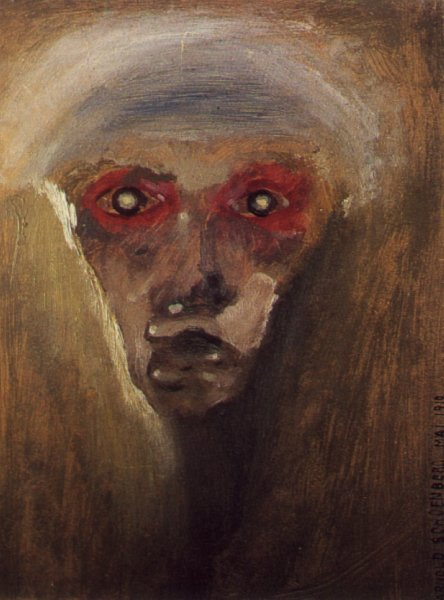
\includegraphics[scale=0.8]{roteblick}\caption{Der Rote Blick - the Red Gaze (1910)}
\label{fig:roteblick}
\end{figure}

Two music dramas followed in quick succession: \textit{Ewartung} (expectation) for soprano and orchestra (1909) and \textit{Die gl\"uckliche Hand} (the lucky hand) for voices and orchestra (1910/13). In \textit{Ewartung} we hear the hidden thoughts of a woman waiting in the forest for her lover (a Pelleas version again). The synopsis is as follows:

\begin{quotation} 
A woman is in an apprehensive state as she searches for her lover. In the darkness, she comes across what she first thinks is a body, but then realises is a tree-trunk. She is frightened and becomes more anxious as she cannot find the man she is looking for. She then finds a dead body, and sees that it is her lover. She calls out for assistance, but there is no response. She tries to revive him, and addresses him as if he were still alive, angrily charging him with being unfaithful to her. She then asks herself what she is to do with her life, as her lover is now dead. Finally, she wanders off alone into the night.
\end{quotation}

The madness of the tortured mind develops further still with \textit{Pierrot Lunaire} of 1912 for voice and small ensemble comprising piano, flute (pic), clarinet (bass), violin (viola) and cello. Whilst many note this piece as pivotal for its use of Sprechstimme (a kind of semi-pitched vocalisation) this piece projects Schoenberg's own fascination with (and suspiciousness of) numbers. 

Who was Pierrot? Pierrot was a pantomime character and is commonly represented as a sad clown. Columbine is the object of his desires; Harlequin the object of hers. Thus again a love triangle with Pierrot originally the object of ridicule but during Symbolist times, the ultra-sensitive loner with only the moon for company.  

The structure of the work is as three times seven poems drawn from Albert Giraud's writings from 1884 (original in French with German translation by Otto Hartleben).  

\begin{table}[h!]
\begin{tabular}{|p{5.0cm}|p{5.0cm}|p{5.0cm}|} \hline
\textbf{Part One} & \textbf{Part Two} & \textbf{Part Three} \\\hline
Mondestrunken (Moondrunk) & Nacht (Passacaglia) (Night) & Heimweh (Homesickness)\\\hline
Columbine & Gebet an Pierrot (Prayer to Pierrot) & Gemeinheit! (Vulgarity)\\\hline
Der Dandy (The Dandy) & Raub (Theft)  & Parodie (Parody)\\\hline
Eine blasse W\"ascherin (An Ethereal Washerwoman) &  Rote Messe (Red Mass) & Der Mondfleck (The Moonspot)\\\hline
Valse de Chopin (Chopin Waltz) & Galgenlied (Gallows Song)  & Serenade\\\hline
Madonna & Enthauptung (Beheading) & Heimfahrt (Barcarole) (Homeward Bound)\\\hline
Der kranke Mond (The Sick Moon) & Die Kreuze (The Crosses) & O Alter Duft (O Ancient Fragrance)\\\hline
\end{tabular}
\caption{Pierrot Lunaire, 1912}
\label{tab:pierrot}
\end{table}

The stark rendition (especially when semi-staged) and the numerological references are well worth further investigation. 

As Schoenberg paired down the notational script of music so to did his works become more conceptual in size. 
His most famous students were Anton Webern and Alban Berg. Although Berg would follow his composition teacher down the serial road, he was always concerned with larger forms which serialism would not sustain. Webern however was not worried about this and as a consequence his complete oeuvre can be found on just three compact discs. 

Schoenberg's later works including the \textit{Variations for orchestra} (1926/28), \textit{Violin concerto} (1934/36), \textit{String quartet No. 4} (1936), \textit{Piano concerto} (1942), \textit{String Trio} (1946)
and the six minute \textit{A Survivor from Warsaw} (1947) are well worth following up. 
 
\section{Berg: Wozzeck}
\begin{itemize}
\item Listen: \url{https://www.youtube.com/watch?v=uUkbjO8dkDI}
\item Reading: \url{http://adrian-moore.staff.shef.ac.uk/teaching/mus126/wozzeck.pdf}
\end{itemize}

Amongst numerous song cycles, key works of Alban Berg (1885-1935) to follow up are:
\begin{itemize}
\item Piano Sonata Op.1 (1907)
\item String quartet Op.3 (1910)
\item Wozzeck Op.7 (1914-22)
\item Lyric Suite (string quartet, 1925-6)
\item Lulu (1929-35)
\item Violin concerto (1935) 
\end{itemize}

Berg's early life was not a happy one. At age 18, his father had died, the family was poor, Alban's health was unsteady, he was not successful intellectually, he was unhappy in love yet had fathered an unwanted child. Berg attempted suicide. 

Berg's early career was heading towards accountancy when he met Schoenberg. He learned his trades quickly and although poor, was gifted an inheritance in 1905 which allowed him to resign his government job in 1906. In Schoenberg's class Berg quickly became friends with Anton von Webern. Webern we know was killed in September 1945, in Mittersill, near Salzburg. He had stepped out of his son-in-law's house for a smoke and was shot by an American soldier. 

Musically Berg and Webern went separate ways: Berg looked to the past, Webern to an uncertain future. Though both men knew the risks they were taking. Egon Wellesz recounts the premiere performance of Schoenberg's Op.10 quartet: (\href{http://javanese.imslp.info/files/imglnks/usimg/3/37/IMSLP22756-PMLP52074-Berg_-_String_Quartet__Op._3__score_.pdf}{score})

\begin{quotation}
The atmosphere in the elegant and old-fashioned Boesendorfer Hall was tense from the beginning ... The first movement had hardly begun when, enraged by the unexpected C in the fifth bar, the music critic named Karpath jumped up from his seat and shouted, ``Stop it!'' Unperturbed, the Rose Quartet went on; but it was in that scherzo that, after a \textit{fortissimo}, the audience started laughing and its laughter drowned out the music. An elderly gentleman sitting in front of Mahler began whistling on a door key. I heard Mahler shouting, ``I'll risk five florins (the fine for disturbing the peace) and box you on the ear!'' ``You are not here as director of the Opera, you can't order me to stop,'' the man retorted. Mahler rose from his seat, but at that moment two young men, pupils of Schoenberg, rushed forward and carried the man out of the hall.
\end{quotation}

By the summer of 1907 Berg had been studying harmony and counterpoint with Schoenberg for over two years and was ready to undertake original composition. After numerous small song cycles, Berg began his piano sonata: a planned three movements. Only one transpired and Schoenberg said that was enough. (\href{http://petrucci.mus.auth.gr/imglnks/usimg/7/75/IMSLP234327-SIBLEY1802.21900.4ff7-39087012041663score.pdf}{score})
For all its chromaticism this work is in sonata form and Bminor. 

We should remind ourselves that Berg and Webern were composing at a time of huge Bruckner symphonies were only 10 years old, Strauss was writing virtuoso tone poems and Mahler was conducting his own symphonies. 
Berg was friends with the artist Gustav Klimt and Klimt was the Damien Hurst of his age. 

Berg's first string quartet was premiered on April 24, 1911, just before his wedding to Helene Nahowski. At this point in his life he took his leave from Schoenberg. 
%%%%%%%%%%%%%%%%%%%%%%%%%%%%%%%%%
\section{Webern: Concerto for nine instruments Op. 24}

\begin{itemize}
\item Listen: \url{https://www.youtube.com/watch?v=vmumBURcHlc}
\item Listen: \url{https://www.youtube.com/watch?v=rIr1xrunnf0}
\item Score: \url{http://imslp.org/wiki/Concerto,_Op.24_%28Webern,_Anton%29}
\end{itemize}
